
\section{Discussion}
\label{discuss}
If we treat RCNN(ResNet) trained with three-channel image as our baseline, we can see that complaint information can increase sensitivity with 1.8\% to 94.5\%, it means complaints do have information which can help diagnosis more accruatly. Meanwhile this information also decrease specificity to 90.1\%, which is not hard to understand cause patients sometimes cannot accurately describe his feelings or even exaggerate his condition. If we add information about age and gender, the sensitivity drops a little bit, but the specificity increases to 95.6\%, which means age and gender add information strongly connected to specificity.

The validation loss and accuracy during training is shown in Fig~\ref{loss}. We can see that in Fig~\ref{loss}, MDDNet can achieve higher accuracy at the first phase of training, but RCNN(ResNet), RCNN(GoogLeNet) and RCNN(ResNet) with single loss perform better after. MDDNet's performance outperforms other methods again after 27000 training step. For RCNN(GoogLeNet), it converge slower and has a lower accuracy in the end. According to Fig~\ref{loss}, we can see that information about age and gender can improve accuracy to 0.7 at the very beginning, it means the dataset we are using must be influenced by some certain distribution. So we count the number of male patients and female patients in healthy cases and pneumonic cases(Table~\ref{malefemale}) and number of patients in different ages(Table~\ref{differentages}). 


\begin{figure*}[t]
    \centerline{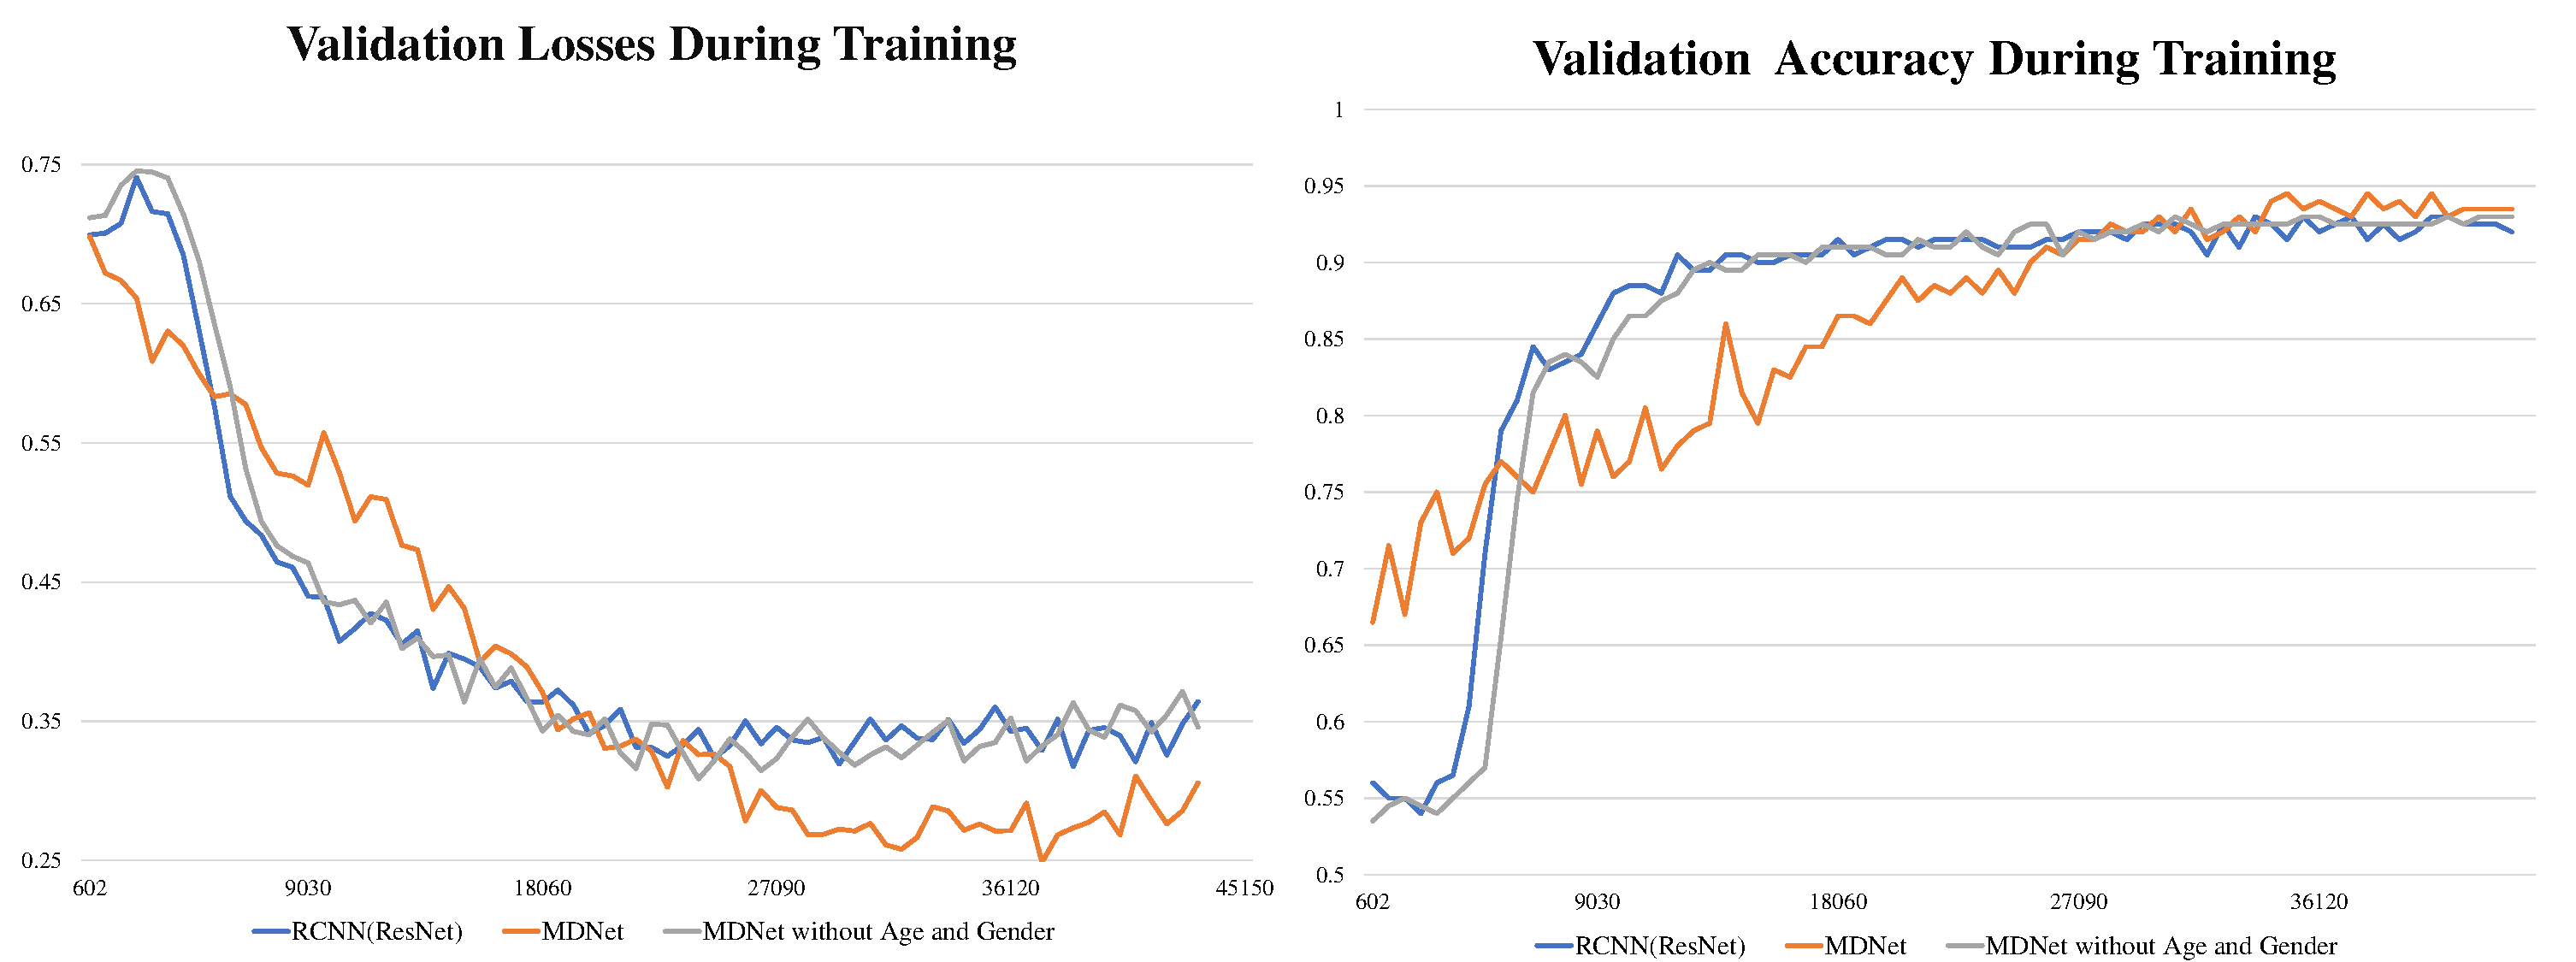
\includegraphics[width=200mm]{losses.pdf}}
    \vspace{-0cm}
    \caption{Validation Loss During Training}
    \vspace{-0cm}
    \label{loss}
    \end{figure*}


In Table~\ref{malefemale}, we can see that a male patient has a larger chance of being pneumonic. In 601 male cases, about 60\% of them are pneumonic, however, in 401 female cases, only 47.6\% are pneumonic. This may be related to smoking since male in Chinese suffer a serious smoking problem. 
In Table~\ref{differentages}, we can see that age is also related to the chance of being pneumonic. We can still observe that people older than 40 have much larger chance of being pneumonic. There are about half of healthy cases between 40-50, but this indication drops so quickly that it goes down to 28.8\% between 50-60. It is not hard to understand this phenomenon, since young people are very sensitive about their healthy condition, they will go to have physical examination as long as they feel uncomfortable, even if they have a lower chance of having pneumonia. However, old people have to face up with another condition. Most old people only go to hospital or clinic when their conditions are very bad. These two tables explain why accuracy can achieve 0.7 at very beginning of training and why information about age and gender can imporve specificity to 95.6\%.


\begin{table}[htb]
    \vspace{-0cm}
    \caption{Number of Male and Female Patients in Healthy and Pneumonic Cases}
    \vspace{-0cm}
    \begin{center}
    \begin{tabular}{|c|c|c|c|c|}
    \hline
    \textbf{\textit{}} & \textbf{\textit{Healthy}} & \textbf{\textit{Pneumonic}}& \textbf{\textit{Total}}& \textbf{\textit{Percentage*}} \\
    \hline
    Male & 240 & 361 & 601 & 60.1\%\\
    Female & 210 & 191 & 401 &47.6\% \\
    \hline
    \textbf{\textit{Total}} & 450 & 552 & 1002 & 55.1\% \\
    
    \hline
    \end{tabular}
    \vspace{0.1cm}
    \label{malefemale} \\
    \footnotesize{Percentage* is Percentage of Pneumonia Patients}

    \end{center}

    \vspace{-0.0cm}
    \end{table}

\begin{table}[htb]
    \vspace{-0cm}
    \caption{Number of Healthy and Pneumonic Cases in Different Ages}
    \vspace{-0cm}
    \begin{center}
    \begin{tabular}{|c|c|c|c|c|}
        \hline
        \textbf{\textit{}} & \textbf{\textit{Healthy}} & \textbf{\textit{Pneumonic}}& \textbf{\textit{Total}}& \textbf{\textit{Percentage*}} \\
    \hline
    0-10 & 6 & 1 & 7 & 14.3\%\\
    10-20 & 31 & 2 & 33 & 6.1\%\\
    20-30 & 122 & 30 & 152 & 19.7\%\\
    30-40 & 124 & 45 & 169 &26.6\%\\
    40-50 & 109 & 108 & 217 &49.8\%\\
    50-60 & 53 & 131 & 184 &71.2\%\\
    60-70 & 5 & 126 & 131 &96.2\%\\
    70-80 & 0 & 82 & 82 &100\%\\
    $>90$& 0 & 27 & 27 &100\%\\
    \hline 
    \textbf{\textit{Total}} & 450 & 552 & 1002 & 55.1\% \\
    
    \hline
    \end{tabular}
    \vspace{0.1cm}
    \label{differentages}\\
    \footnotesize{Percentage* is Percentage of Pneumonia Patients}

    \end{center}
    \vspace{-0.0cm}
    \end{table}


In Fig~\ref{loss}, we can see that RCNN(GoogLeNet) has the highest loss in the end, so it performs the worst in accuracy. RCNN(ResNet) and MDDNet without age and gender has similar performance. RCNN(ResNet) with single loss drops quickly at first, but its loss is very close to RCNN(ResNet) in the end. MDDNet has the lowest loss at the beginning of training, even if it has the highest loss for a moment during training, it has the lowest loss after 27090 training steps. This phenomenon is not hard to understand, since our dataset is influenced by distributions shown in Table~\ref{malefemale} and Table~\ref{differentages}, MDDNet need more time to fit joint distribution between age, gender, visual features and textual features.


